\documentclass{rapportDUETI}

\usepackage{lipsum}

\title{Rapport DUETI Aussenac Baptiste} %Titre du fichier

\begin{document}



%----------- Informations du rapport ---------

\titre{RAPPORT DUETI} %Titre du fichier .pdf
\UE{IUT de vélizy} %Nom de la UE

\elevesdeux{
    Robert \textsc{Byrka} \\
    Victor \textsc{Chardéron}
} %Nom de l'enseignant

\eleves{
    Baptiste \textsc{Aussenac} \\
    Engueran \textsc{Baudry} } %Nom des élèves

%----------- Initialisation -------------------
        
\fairemarges %Afficher les marges
\fairepagedegarde %Créer la page de garde
\tabledematieres %Créer la table de matières

%------------ Corps du rapport ----------------



\section{Introduction} 

Lors de notre entrée à l'IUT, nos chemins était déjà tracés : alternance, puis école d'ingénieur pour la plupart. Tout ça était prévu, jusqu'à la découverte, lors de la deuxième année d'IUT, une aubaine à prendre pour écrire un nouvel avenir tout aussi passionnant, celui dans l'Université du Québec à Chicoutimi (UQAC). Cette ouverture à l'international, loin de la zone de confort que nous avions pu construire, était une expérience à ne pas laisser passer. C'est pour cela que nous sommes partis un an au Québec.
Par ailleurs, l'idée était de se rapprocher des collègues de l'iut, colocataires et amis, dans la gestion de la vie.\\

Nous tenons à remercier les professeurs Mme Barbot, Mme Fancett, pour nous avoir montré ce choix qui n'a déçu personne ici, Mme Ronsse pour nous avoir aidé dans l'administration au début de l'année, tout le corps enseignant de l'IUT de Vélizy qui nous ont permis d'avoir de merveilleux résultats grâce à leurs cours, et bien entendu le corps enseignant de l'UQAC (Eric Dallaire en particulier) sans qui nous ne nous serions pas amusé autant cette année.

Baptiste : Je tiens à remercier Antoine Berthier de m'avoir montré son chemin, qui m'a grandement inspiré pour la suite de mes études. 

\subsection{Objectifs professionnels}

L'objectif de partir à l'UQAC était de faire une double diplomation en ayant le DUETI en France ainsi que le Baccalauréat en Informatique au Canada (qui équivaut à une licence ici). De plus le diplôme canadien permet une continuité du cursus dans le pays. En parallèle, nous avons pu découvrir l'enseignement au sein d'une université nord-américaine, différent du système français.

\subsection{Objectifs personnels}

Pendant cette année, nous avons aussi définis une multitude d'objectifs personnels.
Premièrement, découvrir une nouvelle société et une nouvelle culture ainsi qu'un environnement variant beaucoup de la France (particulièrement en hiver). 
Deuxièmement, nous souhaitions acquérir plus d'autonomie et d'organisation en nous retrouvant dans une situation que nous n'avions jamais connu sur le long terme.
Enfin, nous voulions pratiquer du sport, d'équipe, pour nous rapprocher tout en évoluant notre corps

\subsection{Présentation du rapport}

Ce rapport est composé de deux partie:\newline
Une première partie permettra de décrire précisément l’environnement dans lequel nous avons vécu notre année à l’UQAC; à savoir l’État du Québec, la région de Saguenay-Lac-St-Jean, l’université, et un approfondissement personnel de chacun.\newline
La seconde partie détaillera le projet que nous avons eu au cours de notre deuxième semestre. Nous y développerons autant la partie technique du travail que la partie management de projet.



\newpage

\section{Abstract} 

Lors de mon entrée à l'IUT, mon chemin était déjà tracé : alternance, puis école d'ingénieur. Tout ça était prévu, jusqu'à ce que je découvre, lors de ma deuxième année, une aubaine à prendre pour écrire un nouvel avenir tout aussi passionnant, celui dans l'Université du Québec à Chicoutimi (UQAC). Cette ouverture à l'internationnal, loin de la zone de confort que j'ai pu construire, était une experience à ne pas laisser passer. C'est pour cela que je suis parti un an au Québec.
Par ailleurs, l'idée était de se rapprocher des collègues de l'iut, collocataires et amis, dans la gestion de la vie.

\subsection{Professional issues}

L'objectif de partir à l'UQAC était de faire une double diplomation en ayant le DUETI en France ainsi que le Baccalauréat en Informatique au Canada (qui équivaut à une licence ici). De plus le diplôme canadien permet une continuité du cursus dans le pays. En parallèle, nous avons pu découvrir l'enseignement au sein d'une université nord-américaine, différent du système français.

\subsection{Personal issues}

Pendant cette année, nous avons aussi définis une multitude d'objectifs personnels.
Premièrement, découvrir une nouvelle société et une nouvelle culture ainsi qu'un environnement variant beaucoup de la France (particulièrement en hiver). 
Deuxièmement, nous souhaitions acquérir plus d'autonomie et d'organisation en nous retrouvant dans une situation que nous n'avions jamais connu sur le long terme.
Enfin, cette année était l'occasion

\subsection{Summary of the report}

Ce rapport est composé de deux partie:\newline
Une première partie permettra de décrire précisément l’environnement dans lequel nous avons vécu notre année à l’UQAC; à savoir l’État du Québec, la région de Saguenay-Lac-St-Jean, l’université, et un approfondissement personnel de chacun.\newline
La seconde partie détaillera le travail que j’ai effectué avec mes collègues de l'iut avec qui je suis parti. Nous y
développerons autant la partie technique du travail que la partie management de projet.



\newpage

\section{Environnement d'études}

Avant d'écrire notre point de vue sur la région du Québec, de l'environnement majestueux du Canada et de notre mode de vie, voici un peu d'histoire pour se situer dans le contexte de notre année.\\

L’État du Québec fait exception au sein du Canada, ainsi que sur le continent Américain. En effet c’est le seul État du Canada qui a le français comme unique langue officielle (la province du Nouveau-Brunswick a l’anglais et le français comme langue officiel). Cette exception est liée à l’héritage historique de cette région. En effet le Québec était une colonie de la couronne française de 1534 à 1763 avant que la France ne cède la région aux Britanniques (ainsi que ses possessions en Inde) à la suite de la Guerre de Sept Ans.\\

\insererfigure{images/environnement_etudes/Carte_du_Quebec_au_sein_du_Canada.png}
{8cm}
{Région du Québec}
{Carte du québec au sein du canada}
{2cm}

Les Québécois sont très attachés à cette spécificité et cela se traduit notamment par un fort protectionnisme de la francophonie. Ainsi de nombreuses expressions ou mots dérivés de l’anglais qui sont couramment utilisés en France sont bannis au Québec.Un autre paradoxe est que certaines expressions québécoises sont malgré tout en anglais. Par exemple on ne dira pas « je sors tard du travail ce soir » mais « je sors tard de la job ce soir » Le français ne disparaîtra cependant pas avant longtemps du territoire et il est toujours demandé aux élus politiques fédéraux du Canada de maîtriser les deux langues officielles (ce qu’ils réalisent avec plus ou moins de maîtrise).\\

Montréal est la plus grande ville du Québec (près de 50\% des habitant du Québec vie à Montréal ou dans sa banlieue) et la second plus grande du Canada (après Toronto). Elle est la capitale économique du Québec et la seconde place financière au niveau national. Elle est considérée comme la « Métropole universitaire du Canada » avec six universités et 450 centres de recherche. De plus elle accueille l’une des plus grandes fiertés du Québec : le club de hockey des Canadiens de Montréal qui y a élu domicile dès sa création en 1909. C’est l’un des deux clubs canadiens qui joue dans la ligue de hockey USA.\\

Cependant contrairement à ce que beaucoup pensent Montréal n’est pas la capitale du Québec qui n’est autre que la ville de Québec. C’est à Québec que se trouve le parlement de l’État où sont votées les lois propres au Québec ; notamment sur l'administration de la justice, la santé, l'éducation et le droit. De plus c’est dans cette ville que se trouve l’Université de Laval fondée en 1852 qui est la plus vieille université francophone d’Amérique du Nord et la sixième plus vieille du Canada.
C’est aussi là que se situe le siège de l’Université du Québec qui réunit dix établissements universitaires dont l’UQAC.\\

La ville de Québec est un lieu chargé d’histoire avec notamment ses fortifications qui sont des témoins directs de la présence française mais aussi des tensions entre l’Angleterre et le Québec notamment avec l’ajout de défenses sans l’accord de Londres. Le vieux Québec garde encore aujourd’hui les traces des premiers colons français avec des maisons d’architecture typiquement bretonne et normande.\\

Entre les trois grandes villes (Saguenay, Québec, Montréal) que nous avons pu visiter, nous avons remarqué qu'elles avaient toutes un environnement différent, entre la grande ville à l'ambiance New Yorkaise de ses gratte-ciels, la vieille ville remplie d'histoire et la ville proche de la nature, chacune à sa caractéristique qui la rend belle et riche en découverte.

\subsection{Description du Québec}

    \subsubsection{Un mode de vie "A l'américaine"}

L’une des premières choses que nous avons faites en arrivant était du repérage, nous sommes arrivés sur un site avec de nombreux bâtiments reliés les uns aux autres par des passerelles, une salle de sport, un terrain de football américain, un stade d’athlétisme, beaucoup d’installations sportives, cela nous a ravis et nous pensions déjà aux corps de rêves que nous allions obtenir en plus des connaissances en informatiques et des futures activités qui auront lieu.\\

Le premier jour on nous a annoncé la présence de casier, on avait déjà l’image des casiers vraiment personnalisés et propres à chaque personne, cependant nous avons rapidement compris que ces casiers étaient uniquement présents pour éviter de se balader avec les énormes manteaux d’hiver dans tout le bâtiment.\\

La première soirée étudiante mais pas la dernière, malgré le fait que l'on ne soit pas resté longtemps, nous avons pu constater le nombre de personne important sur le site de l’UQAC, avec 6000 élèves présents pendant cette année, il était compliqué d’accéder aux saucisses et au chamallow avec des files d’attente assez conséquentes.\\

Grâce à la quantité de soirée étudiante et à notre intérêt dans la vie étudiante en réalisant du bénévolat lors de ces PU, nous avons rapidement créé des relations avec de nombreuses personnes appartenant aux divers associations et comités.\\

Qui dit Amérique dit pancake et bacon, nous n’avons pas attendu longtemps avant d’adopter ce style de vie composé de petit déjeuner assez chargé : bacon, pancake, sirop d’érable, ils étaient nécessaires avec les séances de sport qui nous attendais dans la journée, ces petits déjeuner par la disparité entre les horaires de chacun était le seul repas que nous ne faisions pas tous ensemble. \\

Pour continuer sur une lancé gustative, les avis sur le plat appelé "Poutine" constitué de frites, de sauce brune et de fromage (surnommé fromage Couic-Couic par Baptiste à cause du bruit lors de sa mastication) diverge, si Robert et Engueran n'ont pas trouvé ce plat à la hauteur de sa renommé, Baptiste et Victor semble l'avoir apprécié. C'est d'ailleurs lors de notre premier restaurant, une pizzeria, que nous avons découvert la notion de Tips, le pourboire, une coutume relativement limité en France. Il faut savoir qu'au Québec ce pourboire avoisine 15 pourcent du prix du repas, il n'est donc pas négligeable.\\

Avec quatre hommes dans une maison, la quantité de nourriture n'est pas à omettre. Heureusement, nos connaissances Françaises nous ont rapidement conseillé des supermarchés proposant des ventes en quantités importantes, très avantageuses d'un point de vue du rapport quantités/prix. Ils nous arrivaient parfois de réaliser des courses composées d'entre 5 et 6 balluchons de 6kg de viandes pour des prix convenables.

\subsubsection{Le Québec en hiver}

Nous étions parti dans l'optique d'affronter la neige, nous n'avons pas été déçu. Malgré la douce température à notre arrivée qui nous a permis de découvrir les environs pendant le premier mois. Les premières températures négatives n'ont pas attendu notre aval pour débarquer. La première tempête que nous avons affronté nous à quelque peu surpris, visibilité limitée au delà d'un mètre, des quantités de neige assez impressionnantes. A la différence des Français, les Québécois sont préparés pour la neige, des camions gigantesques, des tracteurs, des dé-neigeuses, des saleuses, un armada de véhicule afin de conserver une circulation parfaitement normale même après une tempête considérable.\\

Après avoir réalisé le trajet, nous étions persuadé que nous réaliserons celui-ci durant toute l'année cependant, lorsque les températures ont chutées, le bus s'est avéré être un choix relativement optimisé en comparaison à une montée les pieds dans la neige ou sur du verglas. Un plaisir matinal de saluer un conducteur de bus souriant, agréable et attentif à ses passagers.


\subsection{La région de Saguenay-Lac-St-Jean : recul de la ville et nature}
\begin{figure}[h]

\begin{subfigure}{0.5\textwidth}
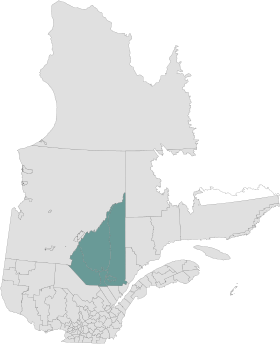
\includegraphics[width=0.9\linewidth, height=8cm]
{images/environnement_etudes/Saguenay.png} 
\caption{Localisation de la régions}
\label{fig:subim1}
\end{subfigure}
\begin{subfigure}{0.5\textwidth}
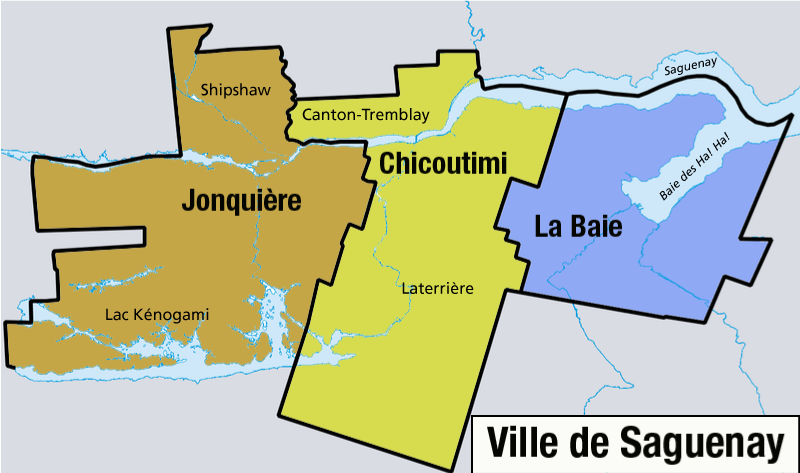
\includegraphics[width=0.9\linewidth, height=6cm]
{images/environnement_etudes/Arrondissements_de_Saguenay.png}
\caption{Arrondissements de la ville de Saguenay}
\label{fig:subim2}
\end{subfigure}

\caption{Saguenay-Lac-St-Jean}
\label{fig:image2}
\end{figure}

L'histoire est qu'avant 2002, la ville de Saguenay n'existait pas, et distinguait les arrondissements en ville.
Centré sur Chicoutimi, fondée en 1842, ce lieu avait une place importante grâce à la vente de fourrure, à son domaine forestier et par l'industrie de l'aluminium. Elle devient aussi une grande place commerciale et administrative notamment avec la construction du palais de justice.
En 1950 l’accessibilité de Chicoutimi est grandement améliorée grâce à la construction du
boulevard Talbot ; route nationale qui relie la ville de Québec à Chicoutimi.


\subsection{L'Université du Québec à Chicoutimi}

L’Université du Québec à Chicoutimi a été ouverte en 1969, elle fête donc ses 51 ans cette année. L’UQAC à été mise en place pour faciliter l’accessibilité aux études dans les régions d’Alma, de Saint-Félicien, de Sept-Îles et de Charlevoix. Elle compte aujourd’hui 7 500 étudiants, et elle propose une soixantaine de programmes au premier cycle, une trentaine au second cycle et neuf doctorats.\\

L’Université est très ouverte à l’internationale. Beaucoup d’étudiants viennent de pays francophones (France, Suisse, Belgique, pays d'Afrique etc…). Nous avons pu remarquer que les étudiants non francophones venaient surtout pour des programmes de troisième cycle.
Beaucoup de professeur viennent aussi de l’étranger.\\

L’Université est constituée de plusieurs pavillons dont les principaux sont :
\begin{itemize}
  \item Pavillon principal où se trouvent :
  \begin{itemize}
      \item Les bureaux administratifs,
      \item Les bureaux des professeurs,
      \item Le centre social (cantine, magasins, locaux des associations étudiantes),
      \item Les principales salles de cours.
  \end{itemize}

  \item Pavillon Alphonse-Desjardins :
  \begin{itemize}
      \item Salles de cours,
      \item Bureau de la rectrice et du vice-recteur,
  \end{itemize}

  \item Pavillon Sportif
  \begin{itemize}
      \item Gymnase,
      \item Salle de sport,
  \end{itemize}

\end{itemize}
Il existe d’autres pavillons notamment les laboratoires de recherche et des bâtiments spécialisés. Il existe des salles spécifiques à certaines activité comme une chambre noire pour le développement de photo ou un studio d’enregistrement.\\

L’Université est construite de sorte qu’en hiver les étudiants n’aient pas à sortir pour aller d’un
bâtiment à l’autre grâce a un réseau de sous-terrains et de passerelles.\\

Il existe au sein de l’UQAC une vie étudiante très dynamique. Ainsi chaque étudiant est inscrit automatiquement dans une association en fonction de sa filière.\\

L’UQAC a beaucoup de sponsors (comme la Caisse des Jardins qui a donné son nom à un bâtiment) pour les différentes constructions et rénovations de bâtiment Elle est l’un des acteur pricipaux de la ville du Saguenay et de sa régions grâce au lien qu’elle a avec les entreprises du secteur. On peut par exemple parler de l’ouverture d’un studio Ubisoft
à Chicoutimi attiré principalement par la qualité des enseignements de l’UQAC en jeux vidéo.\\

On peut aussi parler des nombreux laboratoires de recherche de l’Université qui travaillent avec des entreprises dans différents secteurs comme l’aluminium, le bois ou l’informatique ; les principaux domaines d’emploi dans la région du lac saint-Jean.

\subsubsection{Ambiance}

L'ambiance Québécoise est totalement différente de l'ambiance Parisienne, si en Île-de-France certaines personnes peuvent être stressées, je doute que cela puisse être possible à Chicoutimi, la totalité de l'atmosphère semble être optimisé pour diminuer le stress.

Le sport permettait de se vider la tête tout en acquérant une certaine assiduité sportive, nous sommes tous d'accord pour dire que nos niveaux sportifs respectifs ont largement augmentés. Cette année de sport intensif à raison de 3 à 4 séances de sport par semaines nous a permis d'adopter un style de vie décontractés puisque la majeure partie de notre énergie ainsi que de notre temps libre y été dépensé.

Les québécois disposent d'une capacité en relation humaine avoisinant celle de Robert, aucune difficulté à discuter avec les nouveaux arrivants. Leur facilité à mettre à l'aise était quelque peu déconcertante, en y réfléchissant il est probable que ce fut lié à leur accent très communicatif. 

Malgré un accent divertissant, cela ne nous à pas empêcher de rencontrer quelques français aux travers de diverses activités ( Volley-ball, Salle de sport, Party Universitaire). Et c'est par l'affinité avec certains d'entre eux que nous avons réalisés des soirées plus restreintes et intimes, les différentes parties de loup-garou demeurent d'ailleurs un excellent souvenir. 

De retour en France, nous avons gardé contact avec certains d'entre eux grâce aux réseaux sociaux. Des vacances sont d'ailleurs prévus afin de découvrir le Sud duquel, ces demoiselles sont originaires.

 


\subsubsection{Cours}
Dans cette partie nous allons lister les cours que nous avons eu dans l'année.\\

\textcolor{blue}{8IFG145 Gestion de projets informatiques (3.0 cr.)} \\

Amener à comprendre l'importance d'une bonne gestion de projet pour le succès du développement de projets en informatique et en jeu vidéo. Familiariser avec les différentes méthodologies de développement de logiciels dont les méthodes agiles. Initier aux outils utilisés pour gérer le développement de logiciels. Amener à comprendre la relation entre l'aspect technique et l'aspect gestion. Développer des habiletés de travail en équipe, de communication et d'animation de réunions de production.\\

Les problèmes du développement informatique. Rôle de la gestion des projets informatiques comme partie de la solution. Établissement des exigences et validation. Méthodes de développement traditionnelles. Méthodes agiles: Extreme Programming, Scrum, etc. Choix de la méthode de développement et gestion de projets. Arborescence du projet (WBS). 
Échéancier et outils de gestion de projets. Suivi de projet et coordination. Gestion de la configuration et ses outils. Revues formelles. Assurance et mesure de la qualité. Amélioration de la productivité et sa mesure. Effet de l'importance des données sur le projet, la méthodologie de développement et la gestion du projet. Autres sujets connexes: la gestion des connaissances, apprentissage individuel et organisationnel en gestion de projets; le problème de l'estimation: les métriques applicables; le risque dans un projet: son estimation et sa gestion.\\

\textcolor{blue}{Sécurité des réseaux et du Web (3.0 cr.)}\\

Amener à comprendre les concepts de base de la sécurité informatique et de la protection de l'environnement de travail grâce à des logiciels et des protocoles de sécurité. Faire acquérir une approche pratique de la sécurité dans l'environnement de l'Internet. Concepts de base de la sécurité informatique. Menaces. Vulnérabilité des systèmes. Survol des technologies utilisées en sécurité informatique: cryptographie, cryptanalyse, authentification, confidentialité, codes malicieux, pare-feux, audits, détection d'intrusions, etc.\\

Principes de base pour sécuriser un environnement réseau. La taxonomie d'attaques malicieuses sur les réseaux informatiques. Les faiblesses des protocoles réseaux. Installation et configuration des outils de sécurité réseau. Protocoles de sécurité. Sécurité du Web. Concepts de politique de sécurité pour les réseaux. Étude approfondie des technologies utilisées pour la protection des réseaux informatiques. Sécurité de commerce électronique. Modèles de sécurité des langages de programmation. Vérification des mécanismes de sécurité implantés dans une organisation donnée.\\

\textcolor{blue}{8INF422 Systèmes distribués (3.0 cr.)}\\

Permettre à l'étudiant de maîtriser et approfondir les principes des échanges et de communication des systèmes distribués à base objet, composant et service. Approfondir les notions de protocoles de présentation, de session et d'application. Modèles et architectures des applications réparties: client-serveur, deux-tiers, trois-tiers, peer-to-peer, code mobile, Grid et cloud computing. Plateformes distribuées et types de middlewares. Types de communication : par message, par procédure, et par objet. 
Modélisation d'applications distribuées avec UML. Développement des applications distribuées à l'aide d'un paradigme model-vue-contrôleur, notamment dans le contexte de l'Internet. Traitement du côté client versus traitement du côté serveur, contrôle de session, gestion des formulaires, contrôle des erreurs. Concepts d'applications riches (AJAX). Concept de services Web (SOAP) et de ressources (R).\\

\textcolor{blue}{8INF713 Informatique théorique (3.0 cr.)}\\

Étudier les fondements théoriques de l'informatique afin de comprendre quelles sont les propriétés et les limites des ordinateurs.
Formalisation des notions de problème et de langage. Automates finis, expressions régulières
et langages réguliers. Automates à pile et langages hors-contextes. Machines de Turing,
langages récursifs et récursivement énumérables. Indécidabilité. Réductibilité. Classes de
complexité. Hiérarchies.\\

\textcolor{blue}{8TRD157 Bases de données avancées (3.0 cr.)}\\

Faire connaître les composants avancés des bases de données: bases de données
multimédia (Textes, Images et XML) et bases de données pour le commerce électronique
(centralisées et/ou client/serveur). Introduire aux concepts avancés des systèmes de gestion
de bases de données relationnelles. Initier aux architectures de bases de données impliquées
dans le commerce électronique. Approfondir les concepts de modélisation, de conception,
d'implantation et d'administration de bases de données hétérogènes centralisées ou réparties auxquelles on peut accéder par des applications conventionnelles ou en mode client/serveur (intranet ou Internet).\\

Introduction aux bases de données multimédia: 1) base de données de gestion documentaire:
types de données multimédia, modèle relationnel-objet, requêtes multimédia (ABR, CBR et
CBIR), méthodes de classification, d'indexation et de segmentation des données multimédia.
Particularités des techniques de requêtes, présentation et conception des BDMM texte, image
et XML. Méthodes d'interrogation et de manipulation des bases de données multimédia
(SQL3). Réalisation d'un système d'applications multimédia dans un environnement multi-
analystes et multi-usagers selon une approche centralisée et client-serveur en passant par
toutes les étapes de conception. Problèmes d'intégrité des données. Problématique des bases
de données pour le commerce électronique et stratégies d'accès par intranet ou Internet aux
bases de données de production. Particularités des méthodes d'accès et techniques de protection de l'intégrité des données. Liaison de tables locales clientes avec des tables externes par un protocole normalisé (ex. odbc, ...) ou propriétaire (ex. Net8). Concepts d'importation, d'exportation et d'attache de tables. Stratégies de réplication synchrone et
asynchrone. Configuration d'un environnement répliqué et le concept maître - esclave. Gestion
des collisions et les mécanismes de solution. Règles de répartition des données et des
fonctions dans un environnement client/serveur. Solutions propriétaires et publiques pour la
compatibilité http-html-sql-dbms (ex. PHP, JSS,...).\\

\textcolor{blue}{8INF257 Informatique mobile (3.0 cr.)}\\

Concevoir et développer des programmes informatiques exploitant les technologies mobiles
(ex.: téléphones, tablettes, etc.). Rendre capable d'exploiter efficacement les multiples
senseurs des périphériques mobiles (ex.: téléphones, tablettes, etc.) afin d'offrir des services appropriés au contexte d'utilisation.\\

Composants et caractéristiques d'une application mobile, multithread, interfaces utilisateur,
services, senseurs physiques et logiques, base de données, services basés sur la localisation,
débogage, communication (wifi, Bluetooth etc).\\

\textcolor{blue}{8INF309 Stage-projet I (3.0 cr.)}\\

Appliquer les compétences et les connaissances acquises au développement de systèmes
informatiques en entreprises ou dans une organisation.
Démarche touchant la compréhension du problème posé, analyse du domaine et des besoins,
recherche de solutions, justification de celle retenue, méthodologie retenue, élaboration du
projet, conception du modèle informatique, mise en oeuvre. Production de la documentation
accompagnant les diverses étapes du projet selon les principes du génie logiciel. En
collaboration avec des spécialistes de l'informatique de l'entreprise ou de l'organisation, le
stage ou le projet se déroulera selon les modalités prévues par la direction de programme
sous la supervision d'un enseignant. Dépôt d'un rapport écrit qui fera l'objet d'une évaluation.\\

\textcolor{blue}{8INF334 Modélisation et développement objet (3.0 cr.)}\\

Maîtriser les principes d'analyse et de développement logiciel suivant une méthodologie de
conception des systèmes informatiques orientée objet.
Méthodes d'analyse et de conception orientées objet: modélisation avec le langage UML,
procédures de factorisation de programmes orientés objet, cycle de vie du logiciel, passage de
la conception à l'implantation. Concepts avancés de la méthodologie orientée objet:
frameworks, métaclasses, réflexivité, introspection. Comparaison des méthodes et outils
logiciels orientés objet. Utilisation et application des patrons de conception (design patterns)
dans un contexte applicatif réel. Génération de code : que reste-t-il à coder? Assurance qualité
et techniques de tests de logiciels. Illustration des concepts à l'aide du langage JAVA.\\

\textcolor{blue}{8INF435 Algorithmique (3.0 cr.)}\\

Faire comprendre la notion de complexité du traitement informatique. Étudier les différentes
techniques permettant d'analyser l'efficacité des algorithmes. Rendre apte à concevoir et
implanter des algorithmes efficaces.
Analyse: Complexité de temps et d'espace, notation asymptotique, résolution d'équations de
récurrence. Conception: Algorithmes voraces, méthode diviser-pour-régner, programmation
dynamique, algorithmes probabilistes et parallèles. Problèmes indécidables et intraitables.


\subsubsection{Service aux Etudiants}
Comme nous le disions précédemment, la vie étudiante était très dynamique, cela était possible grâce au MAGE UQAC.\\

\insererfigure{images/environnement_etudes/mage.jpg}
{5cm}
{Logo du MAGE-UQAC}{Logo du Mage-UQAC}
{2cm}

Le MAGE-UQAC est l’association représentant l’ensemble des étudiants de l’UQAC. Sa mission est de défendre et promouvoir les intérêts pédagogiques, politiques, sociaux, économiques, culturels, intellectuels, professionnels et matériels de ses membres.\\
Son chiffre d'affaire pour l'année 2019-2020 est de plus de 2 millions de dollars.\\

Il ne se passait pas un jour sans que nous voyons une institution, ou une activité du MAGE dans l'enceinte de l'université.\\

Nous avons donc été surpris d'avoir vu un service, de cette envergure, aussi actif envers les étudiants, c'est pour cela que nous avons fait des efforts pour faire partie du MAGE-UQAC.\\

Le Mage-UQAC possède tout les services aux étudiants présentés ci-dessous. Et nous commencons avec le bar à l'interieur de l'université : le BAR UQAC.

\insererfigure{images/environnement_etudes/baruqac.png}
{5cm}
{Logo du BARUQAC}{Logo du barUQAC}
{2cm}

C'est à cet endroit que nous voyons le reflet du dynamisme de l'université. En effet, c'est ici que sont organisées les différentes soirées, chaque soir, par une association différente :
\begin{itemize}
    \item Soirée des humouristes le lundi
    \item Soirée d'improvisation le mardi
    \item Soirée UNO / Song pop / Baseball poche ou loup-garou le mercredi
    \item Soirée Universitaire le Jeudi (Party Universitaire)
    \item ETC.
\end{itemize}\leavevmode\newline

Cependant, il existait aussi des retransmission en direct des fameux evenements sportifs américain comme les matchs de la NHL pour le hockey et la finale du Superball pour le football américain.\\

Petite apparté pour indiquer que, la coupe du monde de rugby au Japon n'étant pas retransmise, principalement à cause du décalage Horaire, Baptiste et Victor se réveillaient tot pour pouvoir supporter l'équipe de France sans faire trop de bruit au possible, surtout Baptiste, émotionnellement impliqué.\\

Les jeudis soirs sont organisés les soirées Universitaires qui sont les grandes soirées de la semaine.
10\% des recettes de ces soirées sont reversées à l’association organisatrice.\\
Le MAGE uqac à offert aux étudiants pendant les grandes soirées universitaires des artistes célèbres du Québec ont été invités, nous retenons principalement Fouki, rappeur Québécois, qui a attiré l'attention d'un grand public.\\

L'avantage de ces soirées était de donner l'occasion à des étudiants d'être bénévoles, en aidant à l'organisation de la soirée et en soutenant le personnel du bar. Des tâches étaient attribués aux bénévoles en fonction de leurs envies et disponibilités. l'intérêt pour eux est que la soirée était rémunérée en "FREEBEES", monnaie virtuelle pouvant être utilisé dans les services du MAGE-UQAC tel que le bar, ou la cantine étudiante.\\

\insererfigure{images/environnement_etudes/cantine-logo.jpg}
{5cm}
{Logo de la cantine}{Logo de la cantine}
{2cm}

La cantine étudiante, à ne pas confondre avec la cafétéria, est une épicerie où l'on peut acheter des collations tel que du café, des viennoiseries, des sandwich, etc. Les employés sont tous étudiants et membres du MAGE-UQAC. Comme il n'y avait pas d'autres lieux pour acheter le déjeuner, rapidement, l'affluence pouvait varier de quelques étudiants à plusieurs dizaines d'affamés de café et de ce mystérieux produit qu'est le fromage en grain, une tradition pour les personnes amateurs de fromage sans goût, qui se dénomme aussi le "Couic-Couic", énuméré précédemment.\\

\insererfigure{images/environnement_etudes/caf-logo.png}
{4cm}
{Logo de la cafétéria}{Logo de la caf}
{2cm}

La cafétéria, à ne pas confondre avec la cantine étudiante, est le second endroit où l'on peut manger. Elle est comparable aux cantines françaises, un mini-restaurant, cependant, nous notons que le prix de la nourriture à cet endroit nous semblait excessif, plus ou moins 10\$ le repas, ce qui est très différent des 3\euro{} du CROUS où la qualité était similaire et la quantité était supérieur.\\

Une remarque intéressante est que la plupart des étudiants ramenaient leur gamelle.\\

\insererfigure{images/environnement_etudes/coopsco.jpg}
{4cm}
{Logo de la coopsco}{Logo de la coopsco}
{2cm}

La coopérative étudiante est un magasin général, avec une librairie générale et académique, une papéterie, un rayon d'accessoires informatiques et des objets officiels aux couleurs de l'université.\\

\insererfigure{images/environnement_etudes/repro.jpg}
{3cm}
{Logo de la reprographie}{Logo de la repro}
{2cm}

Il existe aussi une reprographie, situé dans la bibliothèque universitaire, est l'endroit où il est possible d'imprimer tout type de documents.

\insererfigure{images/environnement_etudes/escale.jpg}
{14cm}
{L'escale}{image de l'escale}
{2cm}

Enfin, très récemment, un nouveau pavillon à été construit pendant la session d'automne, nous avons pu voir son évolution jour après jour.\\
L'escale est sortie de terre en décembre, pour remplacer la cantine. Cette opération à pu être aboutie grâce à l'investissement de la STS, compagnie de transport du Saguenay, et de l'UQAC, qui s'élève à plusieurs millions de dollars canadien.\\
Le but étant de permettre d'accroître l'activité économique, et aussi de centraliser les transports vers l'université.\\

Tout les services étudiants ont pour employés les étudiants de l'université, qui comptabilise une centaine de salariés, membres du MAGE-UQAC.\\

\subsection{Évènements de l'uqac}

Au cours de l'année, l'université organise, en plus des activités quotidiennes du soir, des évènements uniques. Nous avons pu participer à plusieurs d'entre eux dont nous retenons principalement le "Novemberfest", qui est un festival étudiant mois important que son homologue "le festival étudiant", se déroulant au printemps.\\

\textit{``
Cette année, Du 5 au 7 novembre 2019, les 8 meilleurs malfaiteurs du Saguenay prennent d’assaut l’Université du Québec à Chicoutimi, forçant les otages des 7 fusions à s’affronter dans diverses activités pendant 3 jours.\\
C’est le moment idéal pour les étudiant·es de faire valoir autant leurs connaissances que leurs talents à travers une compétition sous le
thème des séries télévisées.\\
Chaque fusion d’associations s’occupe de préparer une délégation comprenant le plus grand nombre de membres possible.
Sautez dans vos costumes, « binge watchez » vos séries respectives et préparez vous pour un festival haut en couleurs.
``}\\
\rightline{{\rm --- Cahier d'activité de l'UQAC}}\\

Ce festival dure 3 à 4 jours, il oppose des fusions d'associations de l'université de par des activités sportives et intellectuelles réalisées au cours de cette période. Le thème de chaque année diffère; celui de l'année 2019-2020 se portait sur les séries télévisés.\\

L'université propose également des sorties en fin de semaines, comme une sortie à la montagne pour
skier, ou bien encore naviguer sur le Saint-Laurent pour rencontrer les baleines et les belugas.
De plus, l'uqac est investit dans le développement et la promotion de l'activité économique régionale. ils offrent à ces entreprises des journées dédiées à la découverte de leurs produits en les invitant dans le pavillon principal pour participer à une sorte de salon.\\

(malheureux festival étudiant non existé pour cause de covid)\\
activités sportives accordées aux étudiants (voley ball le vendredi, le basket le dimanche, le rugby, le hockey)


\subsection{La vie dans Chicoutimi : l'histoire d'une collocation et d'une vie hors campus}

Vivre à chicoutimi nous à apporté un nombre incalculable d'expériences 

Liste des activités faites au cours de l'année 
- Voyage à Montréal
- Participation robert vie étudiante
- Bénévolat aux PU
- Québec en Hiver
- Hôtel de Glace
- Chien de traîneaux 
- Randonnées sous la neige
- Tour d'un parc national
- Randonnée en montagne
- Ski alpin
- Ski de fond
- Découvertes Culinaires (rappel poutine "à l'américaine", wapiti, bières locales et mets différents de la culture française)





\newpage

\section{Travail de recherche}

\subsection{Introduction}

Maintenant que nous avons définis notre vie au Québec, nous allons parlé la partie technique de notre année. En effet, nous avions pour but d'enrichir nos compétences techniques dans un autre environnement que le système français, et nous verrons que le résultat est intéressant.
\\
Lors de notre deuxième trimestre, nous avions une matière appelé "Stage-projet" permettant d'utiliser les notions apprises au cours des années précédents sur un projet que nous devions définir. En plus de cela, nous avions l'obligation d'être sous la tutelle d'un professeur souhaitant participer à notre projet.\\

Seul ou en équipe, cette matière est une occasion parfaite pour réaliser un projet qui nous intéresse, nous avons donc décidé de créer une équipe pour un seul projet commun.\\

Après avoir fait l'équipe, nous avons cherché un projet qui nous conviendrait tous, qui toucherait le plus de sujets possible, et qui, par ailleurs, nous plairait le plus !\\

Après quelques temps, nous sommes arrivé à cette conclusion : nous voulions travailler sur un gros projet avec différentes branches. C'est-à-dire, créer un serveur avec une nouvelle technologie pour certains, une interface client web inédite, un système de gestion de base de données, et tout ça dans un système de version de contrôle opérationnel (git). Et c'est ce que le projet suivant nous offre. \\

Voici donc l'intitulé de notre projet : \\

\noindent
{\rule{\linewidth}{0.5mm} }
\begin{center}
\color{red}
    \textbf{Application mobile de calendrier groupé avec une gestion de paiement et d'une messagerie instantanée, géré par Socket et un serveur REST.}
\end{center}
\noindent
{\rule{\linewidth}{0.5mm} }

Ce nom relativement long et complet a fait son effet auprès de notre tuteur ainsi qu'au département informatique. 
\\
À la suite de cela, nous avons demandé à notre professeur favori, \textbf{Eric Dallaire}, de nous accompagner sur le projet, car il était le mieux placé pour participer au projet. De part le fait qu'il nous a donné des cours de Bases de données, et d'informatique mobile, il était le candidat idéal.\\

Après avoir parlé avec lui du projet, avant la période de relâche en décembre; il a accepté d'être notre tuteur de projet et c'est ainsi que nous commencions notre projet officieusement. Nous entamions officiellement notre projet en janvier (début de la session d'hiver, en Janvier) avec une avance par rapport aux autres étudiants, ayant attendu le début de la session pour travailler. 

Et voici comment nous allons présenter notre projet dans ce rapport : 

\begin{itemize}
    \item Dans la partie \textbf{Fonctionnalités} nous verrons le contenu du projet, les opérations qu'un utilisateur de l'application peut faire avec quelques illustrations de notre travail.
    \item Dans la partie \textbf{Outils Utilisés}, Nous parlerons des technologies que nous avons mis en place pour développer notre projet, de la conception à la production et quelques captures de code pour comprendre les enjeux de chacun de ces outils.
    \item Enfin, c'est dans \textbf{Gestion du projet} nous observerons les différentes tâches que nous avons effectués pour gérer au mieux notre projet.
\end{itemize}

\subsection{Fonctionnalités}

Lorsque l'on regarde notre application de loin, il semble que c'est un agenda classique permettant de s'organiser entre les différents évènements et activités. Cependant, son intérêt est de gérer plusieurs calendriers par rapport à un groupe de personnes. liant ainsi les utilisateurs pour faciliter la gestion entre eux. Par exemple, les membres du club de bridge de Chicoutimi peuvent se rejoindre sur un calendrier unique afin de voir les différentes séances d'entraînement, tournois ou bien soirée club chez soi. En plus de cela, les membres du club de bridge peuvent communiquer entre eux via une messagerie instantanée qui est implémentée dans le groupe et enfin, pour chaque évènement, les membres du club de bridge peuvent ajouter des dépenses liées à l'activité et ainsi offrir un équilibre financier entre les participants d'un évènement, pour éviter tout conflit entre les différents membres du club.
\\

Un utilisateur est unique par son login et son adresse mail. il se connecte avec un mot de passe qu'il aura créé lors de son inscription dans la partie "register". De plus, lors de la création du compte, il obtient un calendrier personnel avec le code couleur de son choix. Cependant, s'il désire avoir d'autres calendriers (pour les partager avec d'autres utilisateurs) il peut en ajouter grâce à un titre, une description et un thème qui lui sera demandé par la suite.
Il à la possibilité de rejoindre un calendrier si un membre de ce dernier le lui partage à l'aide d'un lien qui lui serait envoyé. Après avoir entré le lien dans le champs de saisie approprié, le calendrier est ajouté à la liste des calendriers possédés par l'utilisateur et il peut ainsi naviguer entre les différents agendas. 
\\

L'usager souhaitant \textbf{enrichir un calendrier d'évènements} doit simplement se rendre vers le calendrier en question et remplir les zones d'informations tel que le titre, la date de début, la date de fin, incluant l'heure de début et de fin, et une brève description de l'évènement. Il sera ensuite ajouté sur la liste des évènements.
\\
Pendant la partie conception et analyse de notre besoin, nous devions trouver une fonctionnalité qui démarquerait notre agenda des multiples applications qui puissent exister sur le marché.
C'est grâce à notre mode de vie en collocation que nous avons eu l'idée d'ajouter un module de gestion des paiements en fonction d'un évènement. Cette fonctionnalité étant peu représenté dans des agendas, nous pensions qu'il était utile de pouvoir grouper dans une application, un moyen permettant d'observer les dépenses de chacun dans des évènements et de rendre plus facile les remboursements entre les participants

\newpage

\subsubsection{Structure de l'application}

Il est évident que l'application doit avoir une interface afin d'interagir avec un utilisateur. De plus, son rôle est principalement de traiter une grande proportion d'informations (agendas, évènements, comptes utilisateurs, etc, messages), il faut une SGBD avec de solides bases pour être le plus performant. avec Robert nous avons donc réfléchis aux différentes règles que notre structure doit réspecter.
Le plus dur étant que nous n'avions pas de cahier des charges, nous devions, par conséquent, définir les limites de l'application. Et c'est à la suite de plusieurs discussions entre nous que nous avons eu le résultat suivant :

\insererfigure{images/travail_recherche/premier_rendu_structure_bd.png}
{19cm}
{Premier rendu de la structure de la SGBD}
{Première idée de la bd}
{2cm}

Certes sur cette image, petite, nous ne voyons pas vraiment les objets mais elle est plus visible dans la partie \textbf{Annexes}, mais nous observons quand même que notre projet possède assez d'instances pour nous faire travailler.
\\
À la suite de cette première idée de structure de stockage d'informations, nous avons pu parler avec notre professeur tuteur et il nous donna un retour plutôt intéressant, enrichissant pour les étudiants qui souhaitait en savoir d'avantages sur l'architecture et la conception d'une BD.

\insererfigure{images/travail_recherche/photo_reunion_3.jpg}
{17cm}
{Retour du professeur de l'architecture de la SGBD}{
Retour du professeur SGBD}
{2cm}


La communication avec l'application mobile était le point le plus important du projet, car il fallait savoir toutes les données que nous envoyions et que nous devions restreindre.

Nous rédigions donc, à nous quatre, quelques cas d'utilisations que nous montrions au tuteur pendant la première réunion, comme nous pouvons le voir dans le brouillon ci-dessous.

\insererfigure{images/travail_recherche/photo_reunion_1.jpg}
{17cm}
{Élements pour communiquer entre l'application mobile et le serveur}{
Élements pour communiquer entre l'application mobile et le serveur}
{2cm}

\subsubsection{Interface de l'application}
Au début du projet, en parallèle de la conception de la SGBD, Victor et Enguéran ont pu s'occuper de la navigation au sein de l'application mobile, en fonction des scénarii possibles, et nous retenions en premier temps cette navigation possible.

\insererfigure{images/travail_recherche/photo_reunion_2.jpg}
{15cm}
{Retour du professeur après la réunion du premier livrable}{
Retour du professeur Navigation}
{2cm}

C'est sur ses bases, approuvées par le tuteur, que nous avons commencé à réaliser notre interface mobile \footnote{Notez qu'il est possible de voir les illustrations de notre application dans la partie annexe}.\\

Alors que j'administrais avec Enguéran le serveur et la base de données, Robert et Victor concrétisaient le développement de l'application mobile en produisant des fenêtres simples d'utilisation (User-Friendly). Une application mobile ne doit pas être dotée de milliers de boutons, il fallait donc réfléchir aux éléments présents dans chaque fenêtre de manière à ce que l'utilisateur ne se perde pas, et puisse apprécier l'expérience de ce système d'agendas.

\subsubsection{Mécanisme du serveur et de l'application mobile}

Le serveur que nous avons créé était un serveur de REST qui récupérait des requêtes HTTP et qui traitait ensuite les différentes informations qu'un téléphone connecté à internet lui envoyait. Le calcul, et la récupérations des données de la SGBD sont donc fait en arrière plan, de façon distribuée, comme nous l'avions appris en deuxième année de DUT ainsi qu'au premier semestre de l'UQAC. En effet, notre serveur lançait deux applications, Socket et REST, l'un s'opérant pour un canal constant pour accéder aux messages, l'autre pour récupérer de grandes données tel que la liste de tout les événements des calendriers d'un utilisateur.\\

L'application mobile, envoie une multitude de requêtes au serveur. Cette opération permet au téléphone d'afficher uniquement les informations reçues, ce qui le rend fluide et rapide avec son design épuré.


\subsection{Outils Utilisés}
Côté Mobile
-Ionic, Angular = Typescript, technologie nodeJS, HTML, CSS
-Génération d'une application web sur mobile
-Tests des fonctionnalités effectuées sur téléphone android, ios, ainsi que sur le navigateur web des pc

Côté serveur
python, REST, cx\_oracle (libraire pour communiquer avec la SGBD)

Côté SGBD : oracle et sqlmodeller pour la conception (en plus de papier crayon)
Gestion de la base de données avec un script de réinitialisation

Git pour le système de version de projet

Editeur de texte Visual studio code pour comprendre le principe du lancement des programmes (sans ide)

\subsection{Gestion du projet}
2 gits

Kanban avec to do comme trello

Parler pdt la journée des choses à faire

Communication avec le tuteure tout les mois de façon agile en donnant un livrable

Travail sur visual studio code avec le live share : module permettant de coder à plusieurs sur un même fichier, utile pour faire du pair programming qui était une méthode efficace

Baptiste s'occupant de la partie SBGD + serveur ainsi que support pour Ionic,
Enguérant traitant les serveurs, ajoutant des fonctionnalités comme le paiement et un algorithme de réduction de transferts d'argent,
Victor et Robert travaillant Full Stack sur le serveur REST et sur l'interface mobile, et la communication entre le télephone et les serveurs

debuggage et fin d

\subsection{Idées d'implémentation}

Bien sûr, un projet de cette ampleur est ambitieux, une multitude de chemins s'offre à nous pour ce projet.

\subsection{S'adapter avec le virus}

Comme tout les étudiants en secondaire, nous avons du travailler sur le projet pendant la crise sanitaire. 

debbugage et finalisation du projet
\newpage

\section{Conclusion : une fin prématurée qui désole plus d'un}

Le coronavirus ne nous aura pas
\newpage

\section{Annexe}


Liens des projets GIT :\\

\begin{itemize}
    \item GIT pour le serveur SOCKET, REST API et Initialisation à la BD :\\
    \url{https://github.com/BabtuhAuss/projetCalendrierServeur}
    \item GIT pour l'interface IONIC en ANGULAR :\\ \url{https://github.com/BabtuhAuss/projetCalendrierInterface}
\end{itemize}

\vfill

\begin{figure}[H]
    \centering
    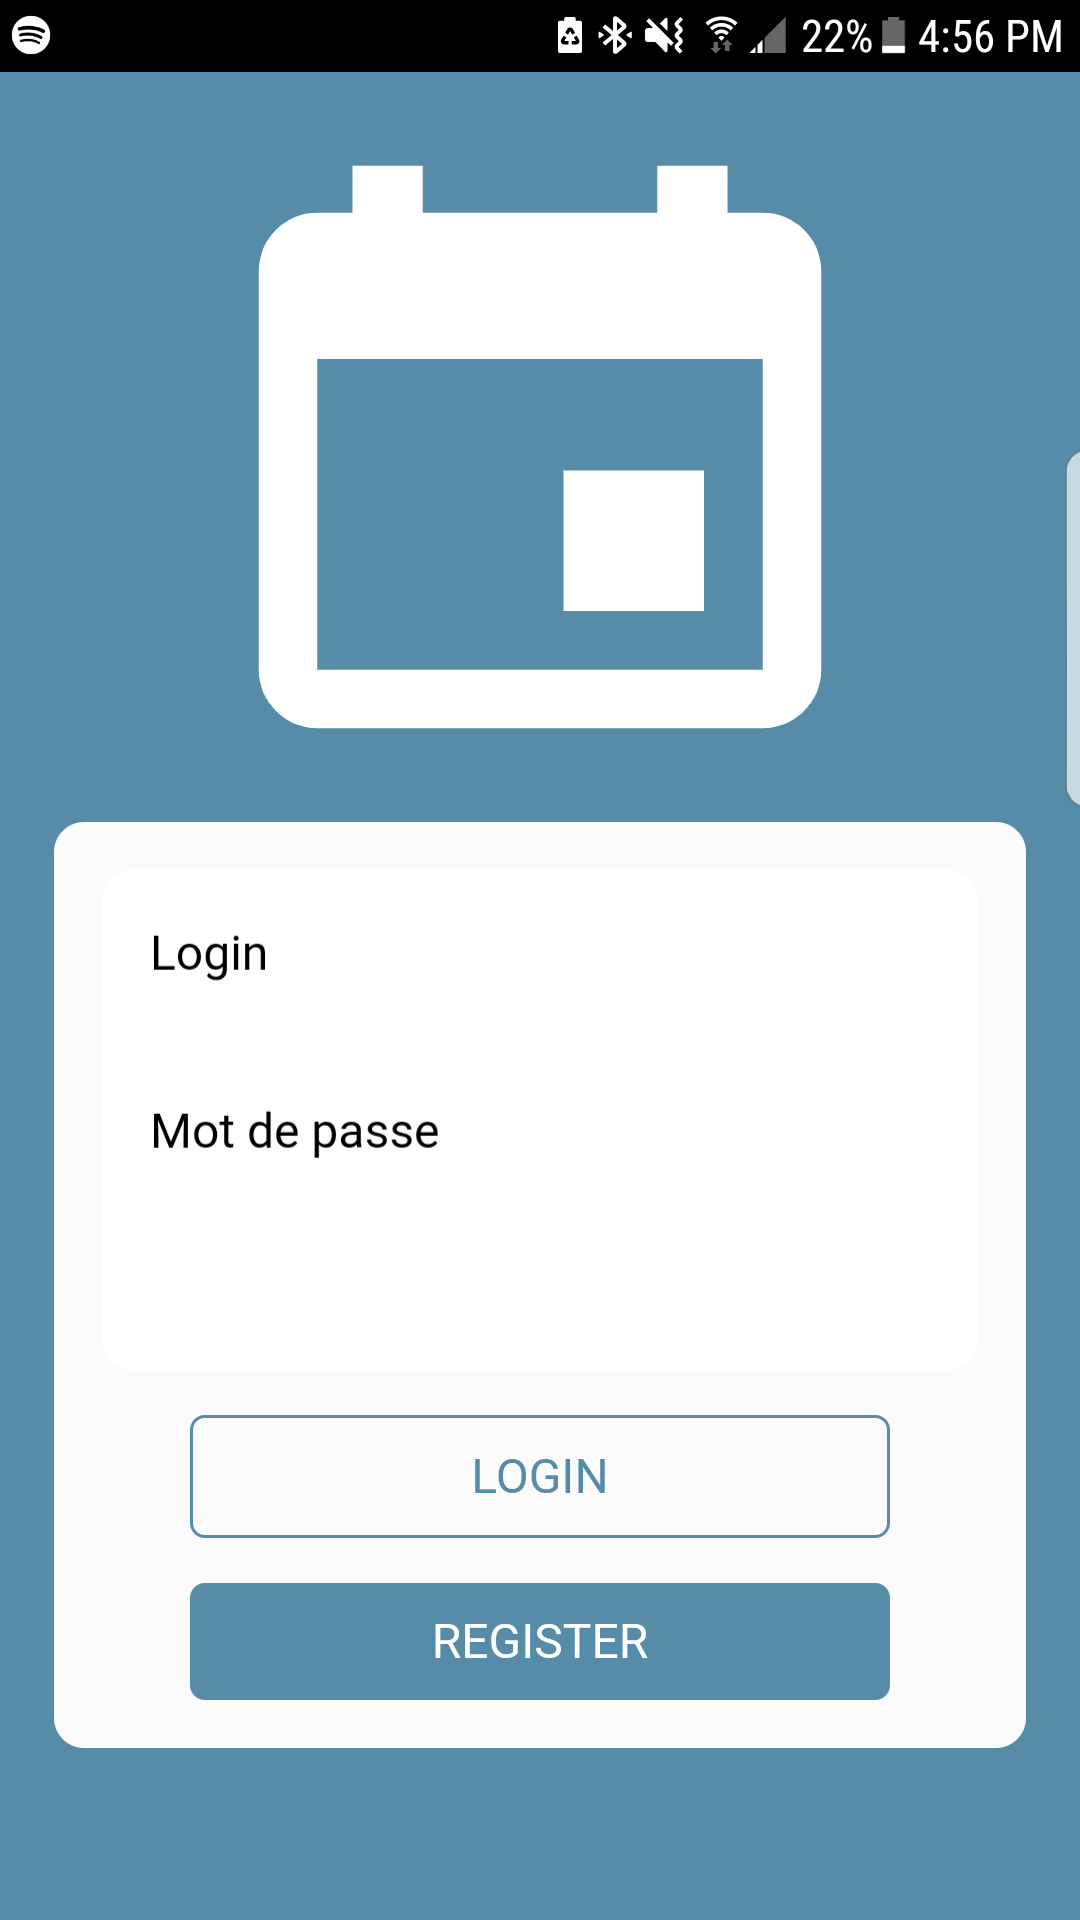
\includegraphics[height=12cm]{Annexe/1.png}
    \caption{Captures d'écran mobile}
    \label{fig:my_label}
\end{figure}

\insertScreenshot



\end{document}
